\documentclass{standalone}
\usepackage{amsmath}
\usepackage[T1]{fontenc}
\usepackage[utf8]{inputenc}

\usepackage[usenames,dvipsnames]{xcolor}

\usepackage{tikz}
\usetikzlibrary{arrows, shapes, matrix}

\begin{document}

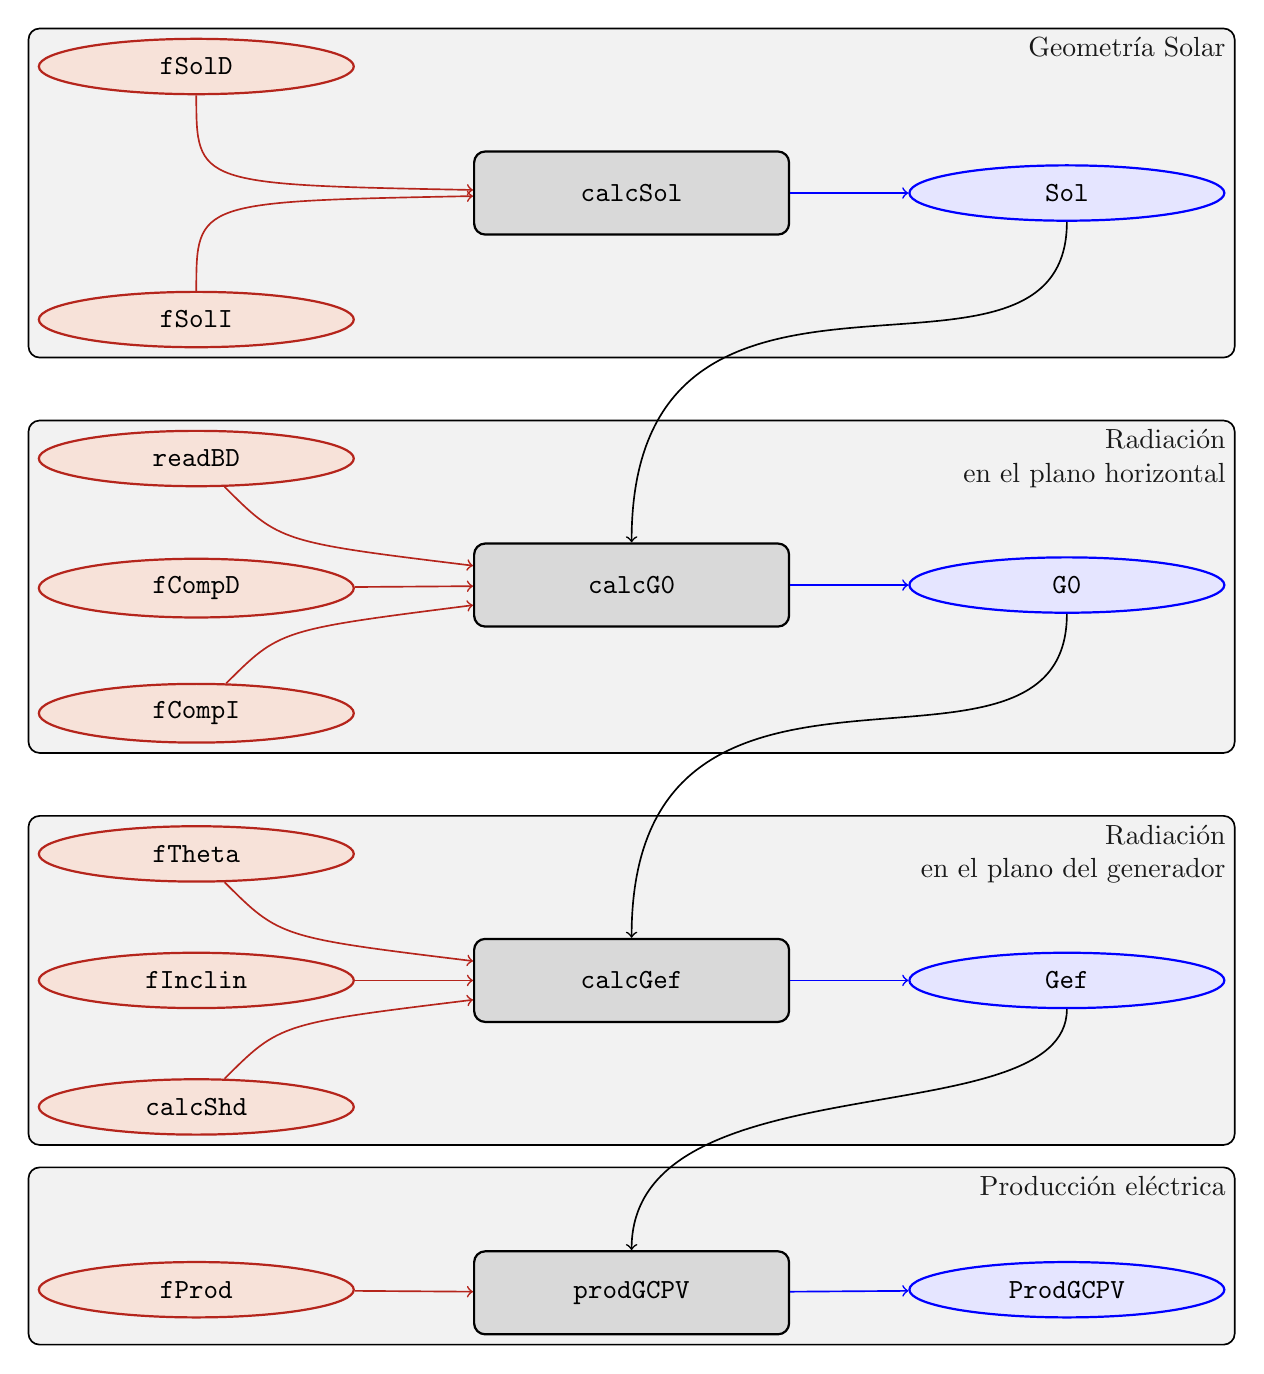
\begin{tikzpicture}[auto,
method/.style={rectangle, rounded corners, draw=black, thick, fill=gray!30,
minimum height=3em, align=flush center, inner sep=1pt},
%
simple/.style={draw=black, circle, fill=gray!30},
%
function/.style ={draw=BrickRed, thick, ellipse, fill=BrickRed!10,
minimum height=2em},
%
class/.style ={draw=Blue, thick, ellipse, fill=Blue!10,
  minimum height=2em, }]

\tikzset{every path/.style={line width=.6pt}}

\begin{scope}
  \matrix [matrix of nodes, rounded corners, fill=gray!10, draw=black,column
  sep=15mm,row sep=7mm, minimum width=4cm] (Geometry) {
    %%%%%%%%%%%%%%%%%%%%%%%%%%%%%%
    \node [function] (fSolD) {\texttt{fSolD}}; &
    \node {}; &
    \node {}; \\
    %%%%%%%%%%%%%%%%%%%%%%%%%%%%%%
    \node {};& 
    \node [method] (calcSol) {\texttt{calcSol}}; &  
    \node [class] (Sol) {\texttt{Sol}}; \\
    %%%%%%%%%%%%%%%%%%%%%%%%%%%%%%
    \node [function] (fSolI) {\texttt{fSolI}}; &
    \node {}; &
    \node {}; \\
  };
\end{scope}

\begin{scope}[yshift=-5cm]
  \matrix [matrix of nodes, rounded corners, fill=gray!10, draw=black, column
  sep=15mm,row sep=7mm, minimum width=4cm] (Horizontal) {
    %%%%%%%%%%%%%%%%%%%%%%%%%%%%%%
    \node [function] (readBD) {\texttt{readBD}}; &
    \node {}; &
    \node {}; \\
    %%%%%%%%%%%%%%%%%%%%%%%%%%%%%%
    \node [function] (fCompD) {\texttt{fCompD}}; &
    \node [method] (calcG0) {\texttt{calcG0}}; &  
    \node [class] (G0) {\texttt{G0}}; \\
    %%%%%%%%%%%%%%%%%%%%%%%%%%%%%%
    \node [function] (fCompI) {\texttt{fCompI}}; &
    \node {}; &
    \node {}; \\
  };
\end{scope}

\begin{scope}[yshift=-10cm]
  \matrix [matrix of nodes, rounded corners, fill=gray!10, draw=black,column
  sep=15mm,row sep=7mm, minimum width=4cm] (Generator) {
    %%%%%%%%%%%%%%%%%%%%%%%%%%%%%%
    \node [function] (fTheta) {\texttt{fTheta}}; &
    \node {}; &
    \node {}; \\
    %%%%%%%%%%%%%%%%%%%%%%%%%%%%%%
    \node [function] (fInclin) {\texttt{fInclin}}; &
    \node [method] (calcGef) {\texttt{calcGef}}; &  
    \node [class] (Gef) {\texttt{Gef}}; \\
    %%%%%%%%%%%%%%%%%%%%%%%%%%%%%%
    \node [function] (calcShd) {\texttt{calcShd}}; &
    \node {}; &
    \node {}; \\
  };
\end{scope}

\begin{scope}[yshift=-13.5cm]
  \matrix [matrix of nodes, rounded corners, fill=gray!10, draw=black,column
  sep=15mm,row sep=7mm, minimum width=4cm] (System) {
    %%%%%%%%%%%%%%%%%%%%%%%%%%%%%%
    \node {}; &
    \node {}; &
    \node {}; \\
    %%%%%%%%%%%%%%%%%%%%%%%%%%%%%%
    \node [function] (fProd) {\texttt{fProd}};& 
    \node [method] (prodGCPV) {\texttt{prodGCPV}}; &  
    \node [class] (ProdGCPV) {\texttt{ProdGCPV}}; \\
  };
\end{scope}


\begin{scope}
   \draw [->, BrickRed] (fSolD) .. controls ++(-90:1.5) .. (calcSol);
   \draw [->, BrickRed] (fSolI) .. controls ++(90:1.5) .. (calcSol);
   \draw [->, Blue] (calcSol) -- (Sol);
   %%%%%%%%%%%%%%%%%%%%%%%%%%%%%%
   \draw [->, BrickRed] (readBD) .. controls ++(-45:1.5) .. (calcG0);
   \draw [->, BrickRed] (fCompD) -- (calcG0);
   \draw [->, BrickRed] (fCompI) .. controls ++(45:1.5) .. (calcG0);
   \draw [->, Blue] (calcG0) -- (G0);
   %%%%%%%%%%%%%%%%%%%%%%%%%%%%%%
   \draw [->, BrickRed] (fTheta) .. controls ++(-45:1.5) .. (calcGef);
   \draw [->, BrickRed] (fInclin) -- (calcGef);
   \draw [->, BrickRed] (calcShd) .. controls ++(45:1.5) .. (calcGef);
   \draw [->, Blue] (calcGef) -- (Gef);
   %%%%%%%%%%%%%%%%%%%%%%%%%%%%%%
   \draw [->, BrickRed] (fProd) -- (prodGCPV);
   \draw [->, Blue] (prodGCPV) -- (ProdGCPV);
%   %%%%%%%%%%%%%%%%%%%%%%%%%%%%%%
  \draw [->, black] (Sol) .. controls ++(-90:3) and ++ (90:5) .. (calcG0);
  \draw [->, black] (G0) .. controls ++(-90:3) and ++ (90:5) .. (calcGef);
  \draw [->, black] (Gef) .. controls ++(-90:2) and ++ (90:3) .. (prodGCPV);
  %%%%%%%%%%%%%%%%%%%%%%%%%%%%%%
  \node [color=black!90, below left] at (Geometry.north east) {Geometría Solar};
  \node [color=black!90, below left, align = right] at (Horizontal.north east) {Radiación \\en el plano horizontal};
  \node [color=black!90, below left, align = right] at (Generator.north east) {Radiación \\en el plano del generador};
  \node [color=black!90, below left] at (System.north east) {Producción eléctrica};
\end{scope}

\end{tikzpicture}

\end{document}
